\section{ساختمان رویداد}
ساختمان رویداد
\lf{Event Structure}
\cite{es}
یک مدل محاسباتی
\lf{Computational Model}
غیر‌جای‌گذاری شده
\lf{Non-Interleaving}
برای پردازه‌های هم‌روند
\lf{Concurrent}
است.
در این مدل، برخلاف مدل‌های جایگذاری شده
\lf{Interleaving}
مانند سیستم‌انتقال که هم‌روندی پردازه‌های موازی با انتخاب غیرقطعی مدل می‌شود، هم‌روندی پردازه‌ها به صورت صریح در مدل توصیف می‌شوند.
\begin{definition}{ساختمان رویداد}
    یک ساختمان رویداد یک سه‌تایی
    $(E,\#,\vdash)$
    است که در آن:
    \begin{enumerate}
        \item $E$
              یک مجموعه از رویداد‌ها است
        \item $\#$
              رابطه‌ی تعارض
              \lf{Conflict}
              ، یک رابطه‌ی دودویی متقارن و غیربازتابی بر روی مجموعه‌ی
              $E$
              است
        \item $\vdash \subseteq Con \times E$
              رابطه‌ی فعال سازی
              \lf{Enabling}
              است که شرط زیر را برقرار می‌کند:
              \begin{align*}
                  X \vdash e \wedge X \subseteq Y \in Con
                  \Rightarrow Y \vdash e
              \end{align*}
    \end{enumerate}
    در رابطه‌ی بالا
    $Con$
    زیرمجموعه‌ای از مجموعه‌ی توانی رویدادها است که اعضای آن فاقد تعارض باشند.
    به صورت دقیق‌تر داریم:
    \begin{align*}
        Con = \s{X \subseteq E| \forall e,e' \in X. \neg(e\#e')}
    \end{align*}
\end{definition}
\begin{definition}
    به ازای هر ساختمان رویداد، می‌توانیم رابطه‌ی فعال‌سازی مینیمال را به صورت زیر تعریف کنیم:
    \begin{align*}
        X \vdash_{min} e \iff X \vdash e \wedge
        ( \forall Y \subseteq X . Y \vdash e \Rightarrow Y = X )
    \end{align*}
    همچنین در هر ساختمان رویدادی شرط زیر برقرار است:
    \begin{align*}
        Y \vdash e \Rightarrow \exists X \subseteq Y . X \vdash_{min} e
    \end{align*}
\end{definition}

برای مشخص کردن وضعیت یک سیتم در هر لحظه از مفهومی به نام پیکر‌بندی
\lf{Configuration}
استفاده می‌شود و
و یک مجموعه شامل رویدادهایی است که تا آن لحظه در سیستم رخ داده‌اند.
\begin{definition}
    اگر
    $\mathrm{E} = (E,\#,\vdash)$
    یک ساختمان رویداد باشد، یک پیکربندی آن یک زیرمجموعه از رویداد‌ها
    $x \subseteq E$
    است که شرایط زیر را داشته باشد:
    \begin{enumerate}
        \item $x \in Con$
        \item $\forall e \in x \exists e_0,...,e_n \in x. e_n = e \ \&
                  \forall i \leq n. \s{e_0,...,e_{i-1}} \vdash e_i$
    \end{enumerate}
\end{definition}
مجموعه‌ی همه‌ی پیکربندی‌های یک ساختمان رویداد مانند
$\mathrm{E}$
با
$\mathcal{F}(\mathrm{E})$
نمایش داده می‌شود.

شبکه‌ی موجود در شکل
\ref{fig:es:update}
را در نظر بگیرید.
در این شبکه دو هاست ۱ و ۲ به صورت هم‌روند یک بسته را به سوییچ ارسال می‌کنند.
این بسته‌ها شامل اطلاعات برای به روزرسانی مسیر‌های دیگر در شبکه هستند، بنابراین سوییچ پس از دریافت هر دوی این بسته‌ها آن ها را پردازش کرده و مسیر‌های خود را به روزرسانی می‌کند.
برای مدل کردن این شبکه می‌توانیم از یک ساختمان رویداد به صورت زیر استفاده کنیم:
\begin{align*}
    \mathrm{E} & = (
    \s{r_1,r_2,u},
    \e, \s{(\e,r_1),(\e,r_2),(\s{r_1,r_2},u)}
    )
\end{align*}
در این ساختمان رویداد، رویداد‌ها به ترتیب دریافت یک بسته از هاست ۱، دریافت یک بسته از هاست ۲ و به روز رسانی سوییچ را مدل می‌کنند.
یکی از روش‌های رسم نمودار برای ساختمان رویداد، رسم نمودار هس
\lf{Hasse}
برای مجموعه‌ی پیکربندی‌های این ساختمان رویداد بر اساس رابطه‌ی زیرمجموعه است.
برای مثالی که بیان شد می‌توان نموداری مطابق شکل
\ref{fig:es:configs}
را رسم کرد.
\begin{figure}
    \centering
    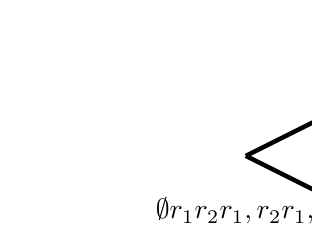
\begin{tikzpicture}[scale=0.8]
        \crd{0}{0}{$\emptyset$}
        \crd[left]{-2}{1}{$\s{r_1}$}
        \crd[right]{2}{1}{$\s{r_2}$}
        \crd[right]{0}{2}{$\s{r_1,r_2}$}
        \crd[right]{0}{3}{$\s{r_1,r_2,u}$}
        \draw [ultra thick] (0,0) -- (2,1);
        \draw [ultra thick] (0,0) -- (-2,1);
        \draw [ultra thick] (-2,1) -- (0,2);
        \draw [ultra thick] (2,1) -- (0,2);
        \draw [ultra thick] (0,2) -- (0,3);
    \end{tikzpicture}
    \caption{}
    \label{fig:es:configs}
\end{figure}

\begin{figure}
    \centering
    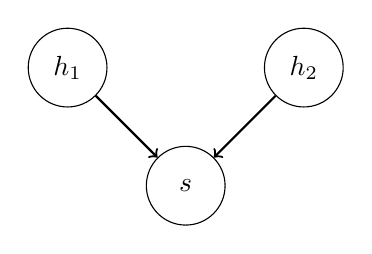
\begin{tikzpicture}[node distance={15mm},minimum size=10mm,
            main/.style = {draw, circle}]
        \node[main] (S)  {$s$};
        \node[main] (H1) [above of=S,left of=S] {$h_1$};
        \node[main] (H2) [above of=S,right of=S] {$h_2$};
        \draw[->,thick] (H1) -- (S);
        \draw[<-,thick] (S) -- (H2);
    \end{tikzpicture}
    \caption{}
    \label{fig:es:update}
\end{figure}